\documentclass[letterpaper,12pt]{article}
\usepackage{graphicx}
\usepackage{booktabs}
\usepackage{pdflscape}
\usepackage{amsmath}
\usepackage{amsthm}
\usepackage{lscape}
\usepackage{enumerate}
\usepackage{float}
\usepackage{bm}
\usepackage{grffile}
\usepackage{relsize}
\usepackage{tablefootnote}
\usepackage{footnote}
\usepackage{sectsty}
\usepackage{xcolor}
\usepackage{caption}
\usepackage{color}
\usepackage{natbib}
\usepackage{multirow}
\usepackage{bbm}
\usepackage[T1]{fontenc}
\usepackage[multiple]{footmisc}
\usepackage{appendix}
\usepackage{times}
\usepackage{relsize}
\usepackage{newtxtext,newtxmath}
\usepackage{enumitem}

%%%%%%%%%%%%%%%%%%%%%%%%%%%%%%%%%%%%%%%%%%%%%%%%%%%%%%%%%%%%
%%%   Title Page Information
%%%%%%%%%%%%%%%%%%%%%%%%%%%%%%%%%%%%%%%%%%%%%%%%%%%%%%%%%%%%
\title{\vspace{-.5in} ECON712: Problem Set 3}
\author{Leandro Freylejer}
\date{Due date: April 15th before noon }

%%%%%%%%%%%%%%%%%%%%%%%%%%%%%%%%%%%%%%%%%%%%%%%%%%%%%%%%%%%%
%%%   Double and Single Space Commands
%%%%%%%%%%%%%%%%%%%%%%%%%%%%%%%%%%%%%%%%%%%%%%%%%%%%%%%%%%%%
\newlength{\defbaselineskip}
\setlength{\defbaselineskip}{\baselineskip}
\newcommand{\setlinespacing}[1]{\setlength{\baselineskip}{#1 \defbaselineskip}}
\newcommand{\doublespacing}{\setlength{\baselineskip}{1.3 \defbaselineskip}}
\newcommand{\singlespacing}{\setlength{\baselineskip}{1\defbaselineskip}}
\renewcommand{\thesubsection}{\arabic{subsection}}

%%%%%%%%%%%%%%%%%%%%%%%%%%%%%%%%%%%%%%%%%%%%%%%%%%%%%%%%%%%%
%%%   Set Margins Here
%%%%%%%%%%%%%%%%%%%%%%%%%%%%%%%%%%%%%%%%%%%%%%%%%%%%%%%%%%%%
\textwidth=6.5in
\textheight=9in
\oddsidemargin=0.10in
\evensidemargin=0.10in
\topmargin=-0.5in

%%%%%%%%%%%%%%%%%%%%%%%%%%%%%%%%%%%%%%%%%%%%%%%%%%%%%%%%%%%%%
%%%   Actual Document Begins Here
%%%%%%%%%%%%%%%%%%%%%%%%%%%%%%%%%%%%%%%%%%%%%%%%%%%%%%%%%%%%%
\begin{document}
\pagenumbering{arabic}



%%%%%%%%%%%%%%%%%%%%%%%%%%%%%%%%%%%%%%%%%%%%%%%%%%%%%%%%%%%%%
\section*{Question II: Instrumental Variables and Returns to Schooling}
%%%%%%%%%%%%%%%%%%%%%%%%%%%%%%%%%%%%%%%%%%%%%%%%%%%%%%%%%%%%%

This question replicates the instrumental variables analysis in Card (1995), following Cunningham's \textit{Causal Inference: The Mixtape} (Chapter 7, Table 57, p.\ 355). Card (1995) studies the returns to schooling using \textbf{proximity to a four-year college} (\texttt{nearc4}) as an instrument for completed years of education (\texttt{educ}), with log wages (\texttt{lwage}) as the outcome. The identifying idea is that individuals who grew up near a college face a lower cost of attending, inducing variation in educational attainment that is plausibly unrelated to unobserved determinants of wages.

\begin{enumerate}[label=(\alph*)]

%%% Part (a): FWL scatter plots + Wald estimate + weak instrument
\item (10 points) Use the Frisch--Waugh--Lovell (FWL) theorem to partial out the included controls and visualize the identifying variation in the data.

\begin{enumerate}[label=(\roman*)]
    \item Let $\bm{X}_c$ denote the matrix of included controls (all regressors except \texttt{educ} and \texttt{nearc4}: experience, its square, \texttt{black}, \texttt{south}, \texttt{smsa}, and region dummies, plus a constant). Regress each of \texttt{educ}, \texttt{nearc4}, and \texttt{lwage} separately on $\bm{X}_c$ and save the residuals $\tilde{d}$, $\tilde{z}$, and $\tilde{y}$, respectively. By FWL, these residuals represent the variation in each variable that is orthogonal to the included controls. \\
\textbf{Answer:} See Log File

    \item Produce two scatter plots, each with a fitted regression line overlaid:
    \begin{itemize}
        \item \textbf{First stage:} $\tilde{d}$ (residualized education) on the vertical axis against $\tilde{z}$ (residualized \texttt{nearc4}) on the horizontal axis.
        \item \textbf{Reduced form:} $\tilde{y}$ (residualized log wage) on the vertical axis against $\tilde{z}$ on the horizontal axis.
    \end{itemize}
    Label your axes clearly and include the slope coefficient of each fitted line on the plot or in the caption.



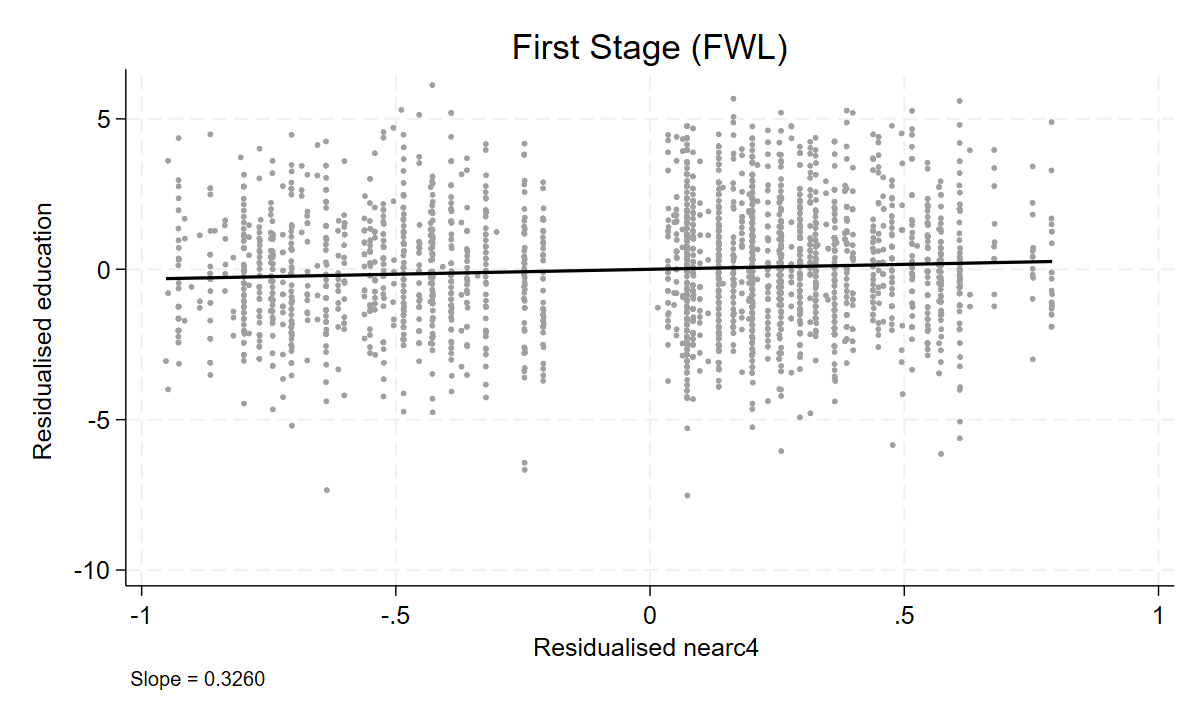
\includegraphics[scale=.3]{PS3_Q2a_FirstStage.png}  



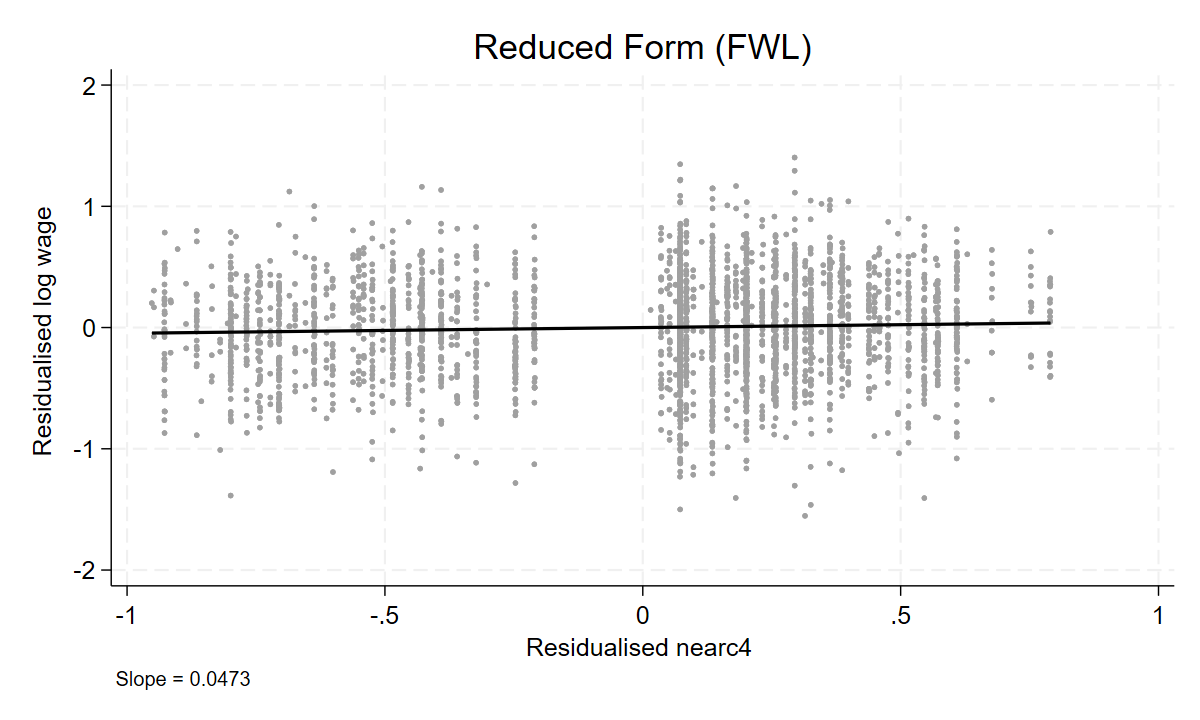
\includegraphics[scale=.3]{PS3_Q2a_ReducedForm.png}


    \item Using the slope coefficients from (ii), compute the Wald IV estimate as:
    \begin{equation}
        \hat{\beta}^{IV}_{Wald} = \frac{\text{slope of reduced form}}{\text{slope of first stage}} = \frac{\tilde{z}'\tilde{y}}{\tilde{z}'\tilde{d}}.
        \label{eq:wald}
    \end{equation}
    Report your estimate \\
\textbf{Answer:}Using the Card (1995) data, the Wald estimate is approximately $\hat{\beta}^{IV}_{Wald} \approx 0.145$, implying that an additional year of education induced by college proximity raises log wages by roughly 14.5\%. 


    \item Using the first-stage regression from (i), report the $F$-statistic on \texttt{nearc4} and comment on whether the instrument appears \textbf{weak}. \\
\textbf{Answer:}
The $F$-statistic on \texttt{nearc4} is approximately $F \approx 15$, exceeding the conventional threshold of $10$.

\end{enumerate}

%%% Part (b): 2SLS replication of Table 57
\item (10 points) \textbf{2SLS estimation (replication of Table 57, p.\ 355).}
Replicate the OLS and 2SLS results reported in Table 57 of \textit{The Mixtape}. Interpret results and compare your 2SLS estimate to the IV-Wald estimate you obtained in part (a)

\begin{table}[H]
\begin{center}
\caption{Replication Table 57}
\resizebox{.57\textwidth}{!}{%
\begin{tabular}{lll}
\hline
\hline
            &         OLS   &        2SLS   \\
educ        &      0.0712***&      0.1242** \\
            &    (0.0036)   &    (0.0492)   \\
exper       &      0.0342***&      0.0556***\\
            &    (0.0023)   &    (0.0199)   \\
black       &     -0.1660***&     -0.1157** \\
            &    (0.0174)   &    (0.0496)   \\
south       &     -0.1316***&     -0.1132***\\
            &    (0.0152)   &    (0.0229)   \\
married     &     -0.0359***&     -0.0320***\\
            &    (0.0036)   &    (0.0051)   \\
smsa        &      0.1758***&      0.1477***\\
            &    (0.0151)   &    (0.0303)   \\
F-test      &               &          17   \\
Observations&        3003   &        3003   \\
$R^2$       &       0.305   &       0.251   \\
\hline
\hline
\end{tabular}}
\end{center}
\captionsetup{font={scriptsize}}
\captionsetup{width=0.80\textwidth}
\captionsetup{skip=0pt}
\caption*{\scriptsize Notes: Heteroscedasticity-robust standard errors in parentheses.
Controls: region dummies, and a constant.
Instrument in 2SLS: \texttt{nearc4} (proximity to 4-year college).
* $p<0.10$, ** $p<0.05$, *** $p<0.01$.}
\end{table}


%%% Part (c): Instrument invalidity
\item (8 points) Describe the conditions under which \texttt{nearc4} would \emph{fail} to be a valid instrument in this setting. Provide at least two concrete, economically plausible channels through which college proximity could directly affect wages independently of years of schooling completed. For each channel, explain the direction of the resulting bias in the 2SLS estimate.\\
\textbf{Answer:}
\medskip
For \texttt{nearc4} to be a valid instrument for \texttt{educ} in the wage equation, it must satisfy:
\begin{itemize}
    \item \textbf{Exclusion restriction:} $\text{Cov}(\texttt{nearc4}_i, \texttt{educ}_i) \neq 0$
    \item \textbf{Strong instrument:} $\texttt{nearc4}_i$ must affect the decision to attend college 
\end{itemize}

\medskip
Channel 1: Areas that have four-year colleges tend to be larger, more urbanized labor markets with a denser set of employers, higher demand for skilled workers, and higher average wages across all education levels.

Channel 2: A child raised near a college town may benefit from higher neighborhood quality, better primary and secondary schools, that translates into higher wages through channels other than completed years of schooling. 

\medskip
In both cases the direction of bias is the same: the instrument is positively correlated with the wage residual $u_i$, so $\hat{\beta}^{2SLS}$ overstates the causal return to schooling.

%%% Part (d): ATE vs LATE
\item (8 points) In words (no algebra required), explain what the 2SLS estimator identifies when the instrument is valid but \emph{heterogeneous treatment effects} are present across individuals. \\
\textbf{Answer:} When the treatment effect of education on wages varies across individuals the 2SLS estimator identifies the Local Average Treatment Effect (LATE). This is the effect on Compliers, who attend college \emph{only because} they grew up near one 

\end{enumerate}

\end{document}
